\documentclass[a4paper,12pt]{report} 
\usepackage{graphicx}
\usepackage{hyperref}
\usepackage{float}

\usepackage{makecell}
\pagestyle{headings}
\graphicspath{{./Images/}}
\hypersetup{
	colorlinks=true,
	linkcolor=blue,
	filecolor=magenta,
	urlcolor=cyan,
}

\begin{document} 
	
\title{Requirement Analysis and Specification Document RASD}
\author{KONG XIANGYI\and ZHANG YUEDONG}
\date{\today}

\maketitle


\tableofcontents



\chapter{Introduction} \label{C1:Introduction}

\section{Purpose}
This document is Requirement Analysis and Specification Document(RASD). The main purpose of this document is the following points
\begin{itemize}
	\item Communicates an understanding of the requirements to the audience and explains both the application domain and the system to be developed.
	\item Contractual: Make this project formal and written so that it has legal effect.
	\item As the baseline for project planning and estimation. i.e. size, cost, schedule. 
	\item As the baseline for software evaluation
		\subitem It can support system testing, verification and validation activities
		\subitem It should contain enough information to verify whether the delivered system meets requirements
	\item As the baseline for change control, such as requirements change, software evolves.
\end{itemize}
And this RASD has the following intended audiences
\begin{itemize}
	\item Costumers \& Users : Some user may interest in validating system goals and high-level description of functionalities.
	\item Systems and Requirements Analysts: The RASD may help them to write various specifications of other systems that inter-relate.
	\item Developers, Programmers: The RASD may help the to implement the requirements
	\item Testers: The RASD may help the to determine that the requirements have been met
	\item Project Managers: The RASD may help them to measure and control the analysis and development processes
\end{itemize}

\section{Scope}
\subsection{Description of the given problem}

At the end of 2019, a global epidemic broke out and swept almost all countries in the world in just a few months. Starting in 2020, people's life rhythm has been completely disrupted by this epidemic, a lot of cities are blocked, people are allowed to exit their homes only for essential needs, everyone had to wear masks and respect the social-distancing at least 1.5 m. In the public area, the human community has to take measures to avoid the crazy spread of the virus. Restaurants began to use dividers to separate the table, supermarkets and museums began to restrict flow of people, the school also adopted into two classes mode: online and onsite.

In this situation, a new problem arises, how to delay the spread of the virus through technical means? 

Since grocery shopping is the most needed activity under the lock-down, so let’s narrow the problem to grocery shopping.

In the supermarket, In order to meet these strict rules, many challenges have arisen, so, we can turn to technology, in particular to software applications, to help navigate the challenges created by the imposed restrictions.

So, this project appeared - Customers Line-up(CLup).

\subsection{World Phenomena}

//TODO ZHANG !!!
\begin{center}
	\begin{tabular}{ c|c } 
		\hline
		$WP_1$ & cell \\ 
		\hline
		$WP_2$ & cell \\ 
		\hline
		$WP_3$ & cell \\ 
		\hline
	\end{tabular}
\end{center}

\subsection{Shared Phenomena}
\begin{center}
	\begin{tabular}{ c|c } 
		\hline
		$SP_1$ & cell \\ 
		\hline
		$SP_2$ & cell \\ 
		\hline
		$SP_3$ & cell \\ 
		\hline
	\end{tabular}
\end{center}


\section{Definitions, acronyms, abbreviations}
\subsection{Definitions}\label{Definitions}
\begin{itemize}
	\item Click Customer : The customer has the required technology to access the store. I.e a smartphone. They can use the customer terminal software.
	\item Brick Customer : The customer doesn't have the required technology to access the store, they have to hand out “tickets” on the spot.
	\item Store Manager : They have to manage the Store System, include the software and hardware.
	\item Ticket: The ticket is a document which contains three key information: QR Code, the estimated departure time, the queue number, and the Store Planned Roadmap. To the click customer, it's \textbf{E-ticket} but to the brick customer,it's \textbf{Paper Ticket},and doesn't contain the estimated departure time, and just a General Store Map without the Planned Road.
	\item QR Code : When customer booked a visit, they will received a QR Code.
	\item QR Code Scanned Machine : A hardware, the Click Customer can use this machine scan their QR code.
	\item Tickets Hand-Out Machine : A hardware, the Brick Customer can use it retrieve their Ticket.
	\item Store Planned Roadmap: A store map that includes a finer way which is recommended form Store System.
	\item Digital Counterpart : A hardware, it with show the queue number.
	\item Store Back-End System : A software, as the back-end manages all stuffs.
	\item On-Time Store Data : A dataset that includes the store's on-time date.
	\begin{itemize}
	\item The current queue 
	\item The customers in the store
	\item The maximum number of people in the store.
	\end{itemize}
	\item Long-Term Customers : The customers with the high average duration of the visit, we set the threshold value to 1 hour.
\end{itemize}


\subsection{Acronyms}
\begin{itemize}
	\item RASD – Requirement Analysis and Specification Document
	\item CLup - Customers Line-up
	\item UI - User Interface
	\item IOS - iPhone OS
	\item PC - Personal Computer
	\item IaaS - Infrastructure as a Service
	\item CRM - Customer Relationship Management
	\item KPI - Key Performance Indicator
\end{itemize}

\subsection{Abbreviations}
\begin{itemize}
	\item  $WP_n$ : n-th world phenomena
	\item  $SP_n$ : n-th shared phenomena
	\item  $R_n$ : n-th functional requirement
	\item  $NR_n$: n-th non functional requirement
	\item  $G_n$ : n-th goal
	\item  $D_n$ : n-th domain assumption
\end{itemize}

\section{Reference documents} \label{Reference documents}
\begin{itemize}
	\item Specification Document: "R\&DD Assignment A.Y. 2020-2021"
	\item Slides of the "Software Engineering 2" course A.Y. 2020-2021
	\item IEEE Recommended Practice for Software Requirements Specifications - IEEE Std 830-1998
	\item  Fondamenti di Sistemi informativi per il Settore dell’Informazione - 7 settembre 2018
	\item Poste Italiane - \url{www.poste.it}
\end{itemize}

//TODO KONG
\section{Overview}
The RASD document consists of different chapters in the structure.\\

\textbf{Introduction}  In the first chapter, it gives the overview of CLup. It provided the definitions, acronyms and abbreviations throughout the document. The description of the product and main goal of this project are provided in the test. 
\\


\textbf{Overall Description} In this chapter, We describe how the product works. In addition, we provide more detailed information about the future details by using well-known diagrams (class diagrams and state diagrams). And product functions gives the more details of requirements. The list of domain assumptions and goals gives the support of the product.  The chapter ends with constrains to customer, manager and store back-end system, which are the basic for proceeding the product.
\\

\textbf{Specific Requirements} This chapter gives a more in-depth and detailed introduction to the system from the aspects of user/hardware/software interfaces, use cases, scenarios, sequence diagrams, and complete mapping of requirements. In use cases, it show the view from the click customer, brick customer and store manager. By using sequence diagram, illustrate the operations between each other. We also provide three small scenarios to explain more details and significant meaningful of CLup, corresponding to the view of click customer, brick customer and store manager. Some specifications regarding performance requirements and design constraints can also be found in the following sections.\\

\textbf{Formal Analysis Using Alloy} In chapter 4, we use Alloy code as the fomal language to model some key concepts and introduce the purpose of it.\\


\chapter{Overall Description} \label{C2:OverallDescription}
\section{Product perspective}

The CLup – Customers Line-up system can divide into three parts. Three client ends and a server end, The client ends are divided into Customer end and Store Manager end according to the object-oriented. Moreover, we have divided Customers into two groups according to their characteristics. We referred to the Business direction's "click and brick" concept in the "\hyperref[Reference documents]{Fondamenti di Sistemi informativi per il Settore dell'Informazione}" teach book, so we decided to name it the "\hyperref[Definitions]{Click Customer}" and the "\hyperref[Definitions]{Brick Customer}", the Click Customer will use the mobile application, and the Brick Customer will use the \hyperref[Definitions]{Tickets Hand-Out Machine} in the store.

The mobile application for the Click Customer can install in the Android and IOS operation system. To make this app simple enough for everyone, we only design two main functions: Sign-up/in and Booking Function. When they book a visit, they have to input four information, the visit date/time, the approximate expected duration of the visit, the categories of items that the Customer intends to buy, and the place they depart. The departing place can input manually by the Customer or recognize by the GPS module. If customers take privacy very seriously, the address can even be fuzzy, as long as it does not affect the calculation of the time to arrive at the store. After they have booked a visit and the Back-End system confirmed it, they will receive the \hyperref[Definitions]{E-Ticket} as soon as possible with four data, QR Code, Queue Number, the estimated departure time and the \hyperref[Definitions]{Store Planned Roadmap}. 

The Tickets Hand-Out Machine is usually placed at the entrance of the store. We design only one button that retrieves a Ticket, no book a visit function. There are two reasons for this design. First of all, this Machina has to easy enough to use. On the other hand, we consider that the Customer going out to pick up the number and wait until the book time to re-come to the store will significantly increase the number of outings, so we did not set up a booking process on this Machine.  Otherwise, we mix the queue of two kind of customer through the \hyperref[Definitions]{Store Back-End System's} queue schedule function to try to best to reduce the wait time.

The Manager end is a Management System that can install on a simple PC. The manager can use it to monitor the \hyperref[Definitions]{Store's On-Time Data}. Furthermore, if there are too many people in some areas or the whole store, the store manager can solve it in two ways. First, he can lower the maximum people value in the store so that the queue will enter slower. On the other hand, he can adjust the queue and let the Customer that will visit the crowded area to enter the store later. After all, if the queue is too long due to these problems, he also can reschedule customers’ book, but he can only reschedule the Customers' booking that before the departure time. 

The most important part of this system is the server end. The server end deployed the \hyperref[Definitions]{Store Back-End System}. This system has to communicate with all other ends and control the Hardware like the Digital Counterpart. It contains three functions, Booking Schedule Function, Queue Schedule Function, \hyperref[Reference documents]{Customer Relationship Management System - CRM System}. The Booking Schedule Function has to communicate with CRM, take the booking data, schedule the booking, and so on... For the Queue Schedule, We refer to the queuing model of the \hyperref[Reference documents]{Poste Italiane}. Its model has already been practiced very maturely. To visit the Poste Italiane, you can book your visit on the Ufficio Postale App or retrieve the ticket on the Machine, and the back-end system will mix two queues reasonably. For our Queue Schedule Function, to achieve goal $G_2$, we have higher requirements. We have to design a better mechanism so that both types of customers do not need to queue for too long, thereby reducing risk. Finally, the CRM System, this sub-system's primary work is communication with the Click Customer's end, like received the booking, integrate all information and generate/send the E-Ticket, by the way, when the Store Manager reschedules the booking, send notification and update the E-Ticket for the Customer. Otherwise, it also does other works like the CRM system usually do. For example, store Customer's data, analyze the Customer's history duration, and mark if this Customer is  \hyperref[Definitions]{Long-Term Customers}.


\subsection{Class Diagram and State Diagram}
\subsubsection{Class Diagram}
The Class Diagram model as shown in Fig.\ref{Class Diagram}, These classes implement the three functions of the Store Back-End System,the Customer Relationship Management sub-System composed by the  Customer class, Booking, Ticket, and CRM class, Among them, the CRM class is responsible for communicating with other ends,and it can control customer class's status,the Customer data will store in Database. The BookSchedule class implement the Booking Schedule Function, all booking data will store in database, and this class can control them. The last class is the QueueSchedule class, it will implement the Queue Schedule Function, it will take booking information and get Brick Customer's ticket information to schedule the queue, the store manager can check the length of the queue and the maximum number of customer in-store, when he found that somewhere in the store was too crowded, he can lower the maximum value. The CallNextCustomer method will control the \hyperref[Definitions]{Digital Counterpart} to make it display the next customer's queue number according to the maximum number allowed in the store. In summary, these functions form a set of effective mechanisms to achieve the goals.



\subsubsection{State Diagram}
The State diagram Fig.\ref{State Diagram 1} illustrated the processing of a customer to require the E-ticket. Customers first register on the CLup, after they will book an appointment and specify their information(time, date, desired goods, etc.), then the can receive an E-Ticket. They can go to the supermarket according to the expected departure time given by the application, and enter the store with E-ticket.
\\ \hspace*{\fill} \\
The State diagram Fig.\ref{State Diagram 2} showed us how the manager monitors Store's On-Time data. The manager can view it on web in computer, and he can know the number of people inside and outside the store. He has the right to adjust the max people number inside the store to balance the capacity of supermarket. In advance, if too many people waiting outside the store, he can also send the notification to the customer who hasn't departed yet.
\\ \hspace*{\fill} \\
The State diagram Fig.\ref{State Diagram 3} represented the serve end proceed various requirements. It receive the registration data and booking information from customers, analyzed customer data (duration time, desired products, categories, etc.) and calculate the route time from users' department place to the store. After the system will optimize the queue order to save everyone time. On the end, the system will generate an E-Ticket in PDF and send it to the user.\\




\begin{figure}[H] 
	\centering
	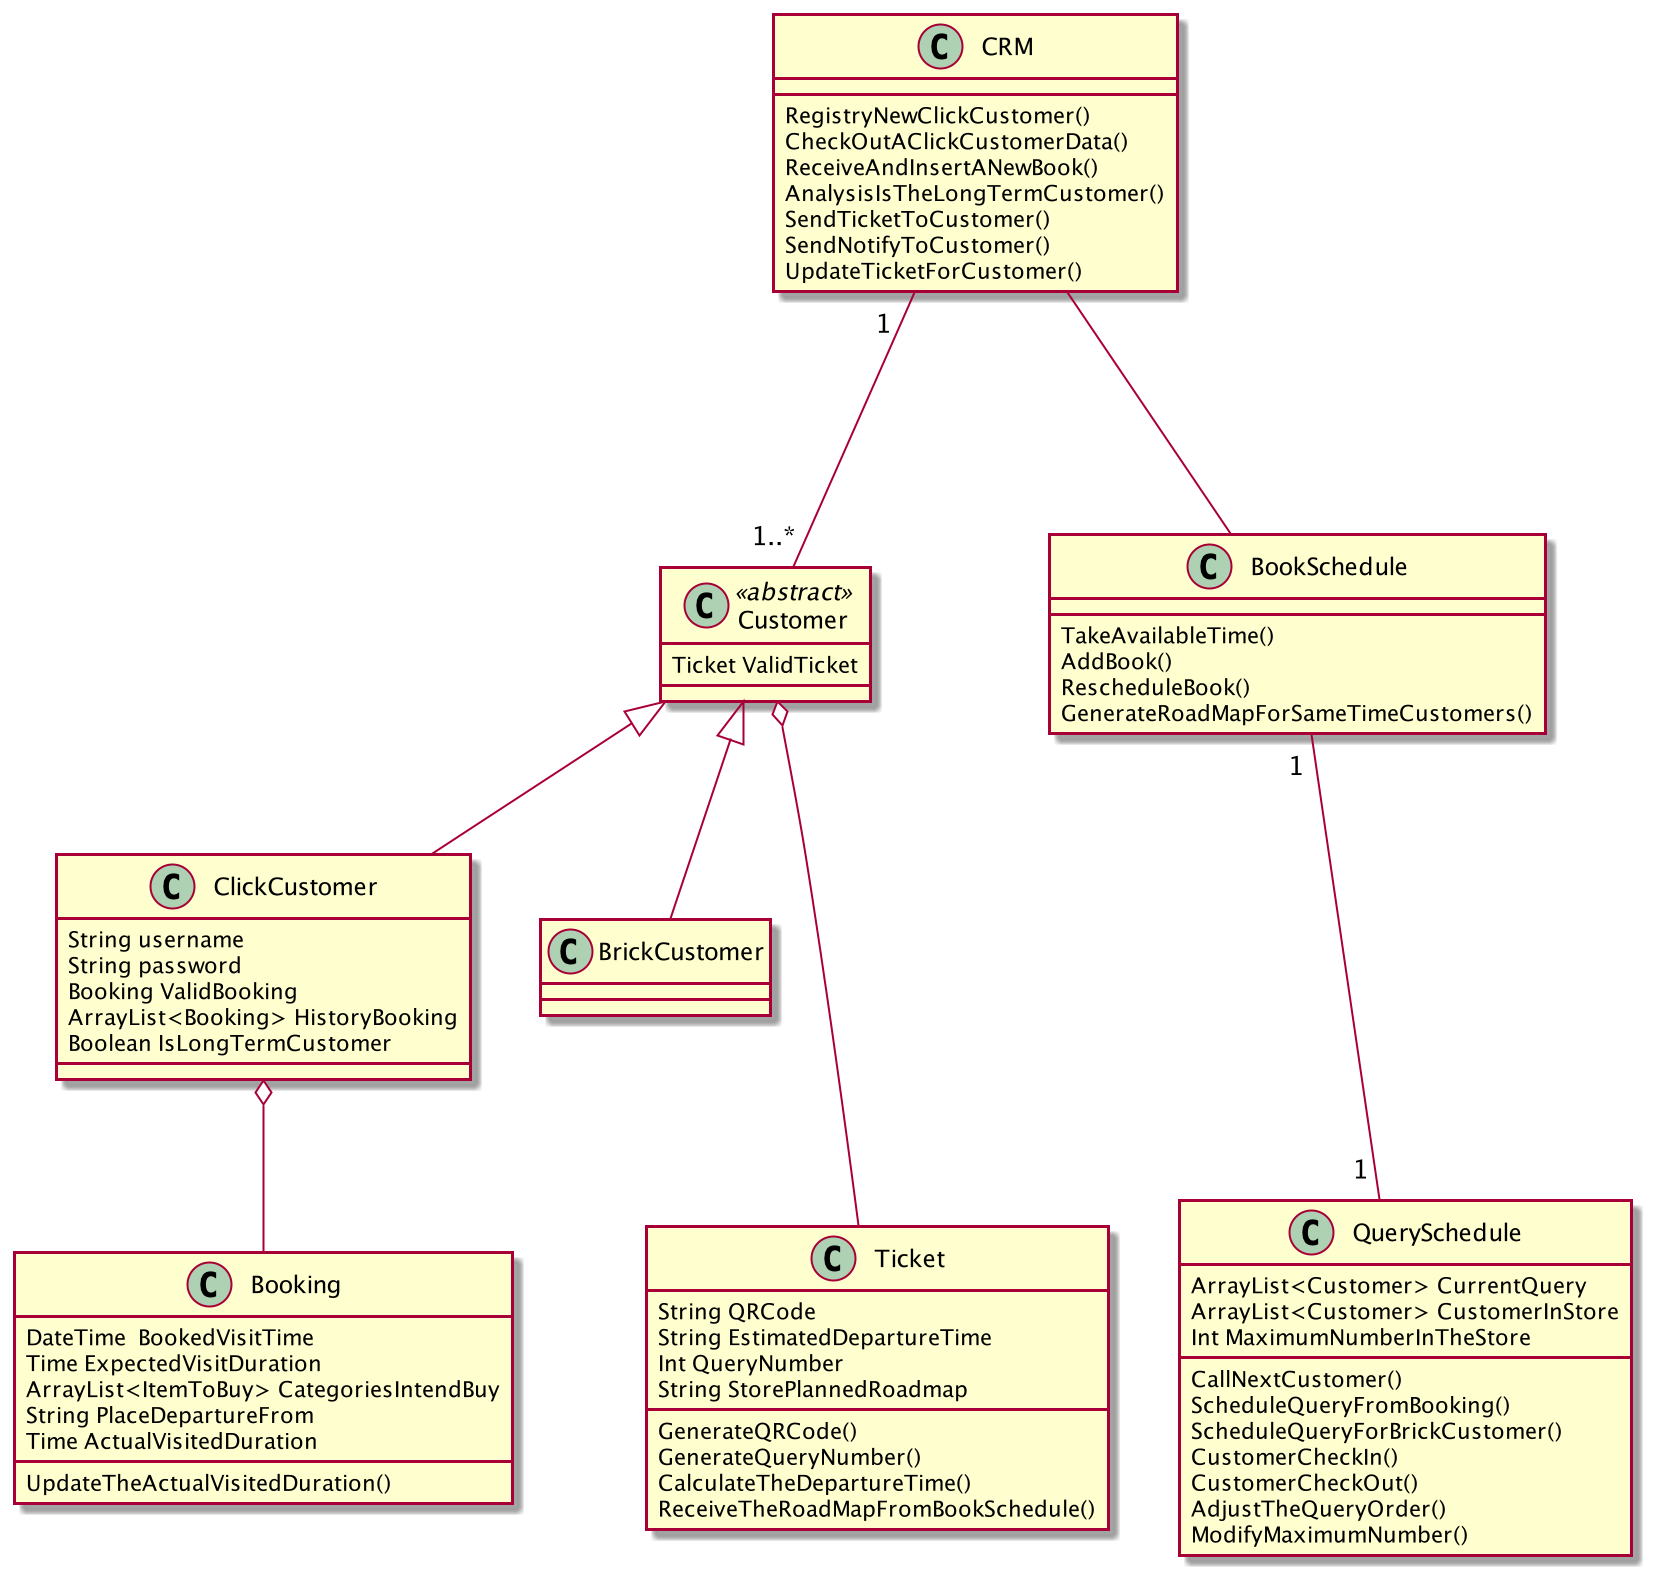
\includegraphics[scale=0.3]{class_diagram.png}
	\caption{CLup Class Diagram}
	\label{Class Diagram}
\end{figure}

\begin{figure}[H]  
	\centering 
	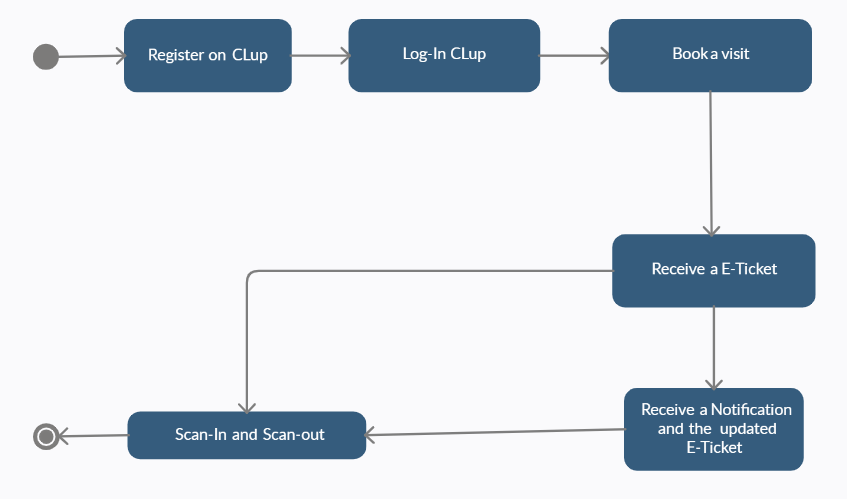
\includegraphics[scale=0.62]{State_diagram1.png}
	\caption{Customer State Diagram}
	\centering
	\label{State Diagram 1}
\end{figure}

\begin{figure}[H] 
	\centering
	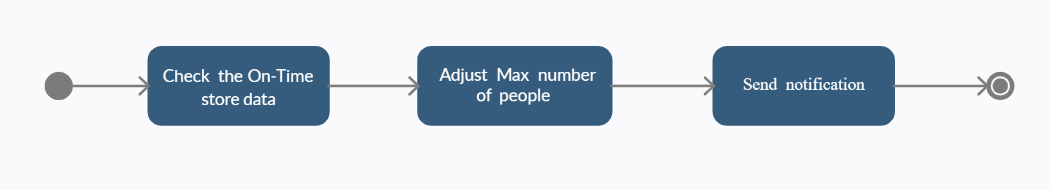
\includegraphics[scale=0.62]{State_diagram2.png}
	\caption{Store Manager State Diagram}
	\centering
	\label{State Diagram 2}
\end{figure}

\begin{figure}[H] 
	\centering
	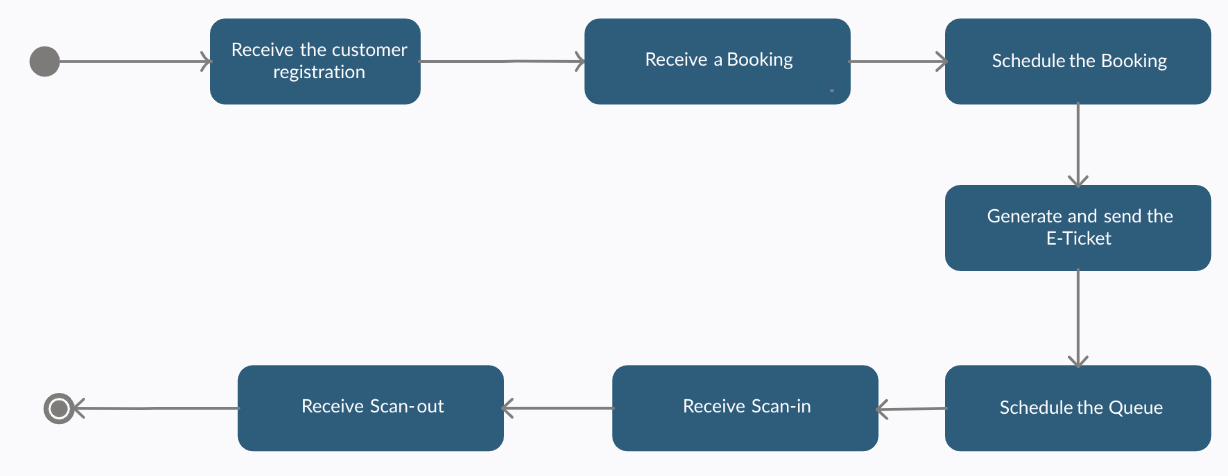
\includegraphics[scale=0.62]{State_diagram3.png}
	\caption{Server End State Diagram}
	\centering
	\label{State Diagram 3}
\end{figure}


\newpage

\section{Product functions}
\subsection{Functional Requirements}
\begin{itemize}
	\item Each \hyperref[Definitions]{Click Customer} shall be able to: 
	\begin{itemize}
		\item Sign-up 
		\item Log-in
		\item Book a visit,to complete it, they have to indicate the following data
		\begin{itemize}
			\item Indicate the desired date and time
			\item Indicate the approximate expected duration of the visit
			\item Indicate the categories of items that they intend to buy
			\item Indicate or given by GPS the current place they want to depart to the shop
		\end{itemize}
		\item Check on the \hyperref[Definitions]{E-Ticket} 
		\item Check on the notification from store manager when their book is rescheduled.
		\item The customer can scan the QR Code at \hyperref[Definitions]{QR Code scanned machine} when they enter \textbf{and} leave the store.
	\end{itemize}

	\item Each \hyperref[Definitions]{Brick Customer} shall be able to
	\begin{itemize}
		\item Retrieve the \hyperref[Definitions]{Ticket} from the \hyperref[Definitions]{Tickets Hand-Out Machine} and wait for the \hyperref[Definitions]{Digital Counterpart} to call them.
		\item Scan the QR Code at QR Code Scanned Machine when they enter \textbf{and} leave the store.
	\end{itemize}

	\item \hyperref[Definitions]{Store Manager} shall be able to: 
	\begin{itemize}
		\item Check out the \hyperref[Definitions]{On-Time Store Data}.
		\item Adjust the maximum number of people in the store.
		\item Adjust the order of the queue.
		\item Check and reschedule the booking.
	\end{itemize}

	\item The \hyperref[Definitions]{Store Back-End System} shall be able to:
	\begin{itemize}
		\item Send the available time/date to the the click customers.
		\item Received and schedule the click customers' book. The scheduling must refer to the duration time of each customer and the categories of items that the customer intends to buy
		\item Calculate the time from the click customer's departure place to the store and put the estimated departure time on the E-Ticket.
		\item Plan and put the Store Planned Roadmap on the \hyperref[Definitions]{E-Ticket}
		\item Send the  E-Ticket to the click customers.
		\item Send a notification and update the E-Ticket to the customer when their book is rescheduled.
		\item Store the customer's data,include:
		\begin{itemize}
			\item Username
			\item Password
			\item Valid Booking data
			\item History visit data.
			\item Is long-term customers
		\end{itemize}
		\item Analysis the history visit data and mark the \hyperref[Definitions]{Long-Term Customers}.
		\item Calculate and store the \hyperref[Definitions]{On-Time Store Data}.
		\item Schedule or reschedule the queue order from the click customer's book and the brick customer's retrieved Ticket.
		\item Control the \hyperref[Definitions]{Digital Counterpart} and display the queue number.
		\item Receive the information from the \hyperref[Definitions]{QR Code Scanned Machine}.
		\item Receive the information from the \hyperref[Definitions]{Tickets Hand-Out Machine}.
	\end{itemize}
\end{itemize}

\subsection{Non-Functional Requirements}
\begin{itemize}
	\item The time from the click customer's departure place to the store that calculates from the \hyperref[Definitions]{Store Back-End System} be precise enough to avoid the Customer arriving at the store too early/late.
	\item The Store Back-End System must schedule the queue reasonably to minimize the wait time.
	\item The Store Back-End System must mix the book and brick customer's retrieved ticket reasonably to allow the click customers to enter the store near the book time by avoiding making the brick customers wait too long.
	\item Cause everyone needs to do grocery shopping, the software for the click customer should be simple enough to use.
\end{itemize}


//TODO ZHANG
\section{User characteristics}
The system will include three categories of user, each of them with different needs:
The Click Customer:
The Brick Customer:
The Store Manager:


\section{Assumptions, Dependencies, and Constraints}

\subsection{Domain Assumptions}
\begin{itemize}
	\item $D_1$ : Everyone will leave the departure place at the departure time indicated by the system.
	\item $D_2$ : Everyone who leaves on time can arrive at the store on time.
	\item $D_3$ : After shopping, everyone can leave the store in time according to their estimated time.
	\item $D_4$ : If something unexpected happens, the store manager can adjust the maximum number of people in the store or reschedule the queue \& customer's book reasonably.
	\item $D_5$ : If someone’s book is rescheduled, he can find the notification in time and set off according to the updated E-Ticket.
	\item $D_6$ : Everyone can consciously scan the QR code at the entrance and exit.
	\item $D_7$ : Everyone can follow the \hyperref[Definitions]{Planned Roadmap} in the store.
	\item $D_8$ : If is possible, everyone tries to best book the visit by the software(be a \hyperref[Definitions]{Click Customer}) instead of picking up tickets on the spot(not be a \hyperref[Definitions]{Brick Customer}).
\end{itemize}

\subsection{Goals}
There are only three main goals of this system.
\begin{itemize}
	\item $G_1$ : Allows store managers to regulate the influx of people in the building.
	\item $G_2$ : Saves people from having to line up and stand outside of stores for hours on end.
	\item $G_3$ : The application plan visits in a finer way to allow more people in the store, at the same time, let the customer occupy different spaces in the store to keep enough distance between them.
\end{itemize}

\subsection{Constraints}
There are not many constraints on the Customer's device. They only need a smartphone with the Android or IOS operation system. When they book a visit, the smartphone has to connect with the Internet. At other times, no need for a stable internet connection. They only need to be able to connect to the Internet discontinuously to receive notifications that may appear.
The manager needs a PC with a stable network connection.
For the \hyperref[Definitions]{Store Back-End System}, we buy an Amazon EC2 IaaS to implement this system.

\chapter{Specific Requirements} \label{C3:SpecificRequirements}

\section{External Interface Requirements}
CLup can be used by the customer who has ability to use smart cellphone. The system will
collect data, analyze the data and create the 'Ticket'. Common users can interface themselves with CLup through a mobile application, the manager has ability to access the system’s functionalities in mobile application or web-based dashboard. Here is shown every kind of
interface that the front-end offers or needs to interact with the users and the back-end.
\subsection{User Interfaces}
In this section there are mock-ups of the user interfaces for the mobile application used
by customer.\\

\textbf{Login} In the Login page Fig.\ref{UI-Login} there are text fields for entering email and password in order to access the personal profile. In case that the customer don't have an account, there is also the option to sign-up.\\

\textbf{Sign-up} In login page Fig.\ref{UI-Register}, the application requests the user to insert the name, email address and a password to register to the system.\\

\textbf{Homepage} Once registered, the user will be welcomed by the homepage Fig.\ref{UI-Home}, that shows the optional of booking, ticket and notification. From booking, users can go to book an appointment for visiting the supermarket. In tickets button, customers can view all their tickets(ticket history, current ticket and up-coming ticket). As for notification part, if users has an unread notification, there will be a red point shown on the right top, after the user read it, the red point will disappear. With this, if users' appointment has been rescheduled by the manger, they can easily receive the notification or message from the manager.\\

\textbf{Booking} After the user enter the booking button, users can see the page Fig.\ref{UI-Booking}, customers need to choose time and date from the given selection. Meanwhile, they need to approximate their duration time and what to buy in the supermarket. On the end, there are two ways to insert the depart address: one is manually insertion of the address by customer, another one is automatic positioning by GPS.\\

\textbf{Category} In this page Fig.\ref{UI-Category}, there are lists of product categories in the supermarket, the product categories corresponding to the different zone in supermarket. Users can choose one or more categories which they want to buy during the shopping.\\ 

\textbf{Manager Dashboard} In the manager dashboard Fig.\ref{UI-Dashboard}, the supermarket manager can see the number of people both inside and outside of the supermarket. He has the right to control the \textbf{Max} number of people inside the supermarket. If too many or too few people in the same zone of the supermarket, he can click 'Adjust', after he can change the max number of people inside the supermarket. And also if too many people waiting outside the supermarket, he can click the 'Reschedule' button, to reschedule the ticket and send the notification to customers who haven't departed yet.\\ 

\begin{figure}[H]
	\begin{minipage}[t]{0.5\linewidth}
		\centering
		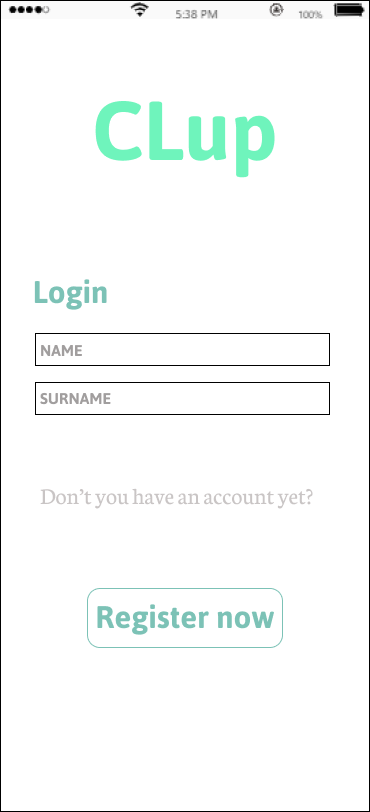
\includegraphics[scale=0.5]{UI-Login.png}
		\caption{UI-Login}
		\label{UI-Login}
	\end{minipage}%
	\begin{minipage}[t]{0.5\linewidth}
		\centering
		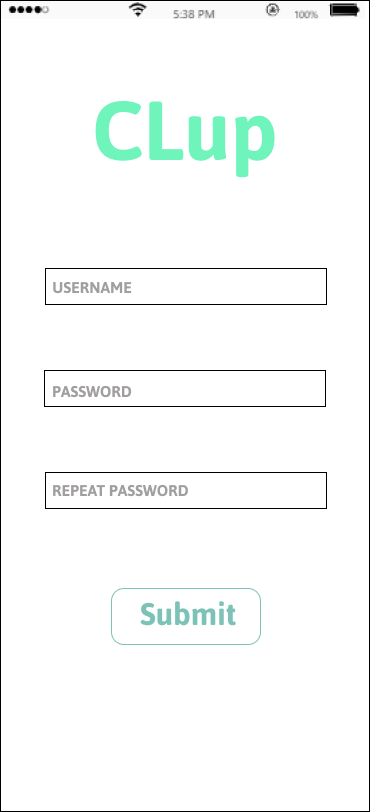
\includegraphics[scale=0.5]{UI-Register.png}
		\caption{UI-Register}
		\label{UI-Register}
	\end{minipage}
\end{figure}

\begin{figure}[H]
	\begin{minipage}[t]{0.5\linewidth}
		\centering
		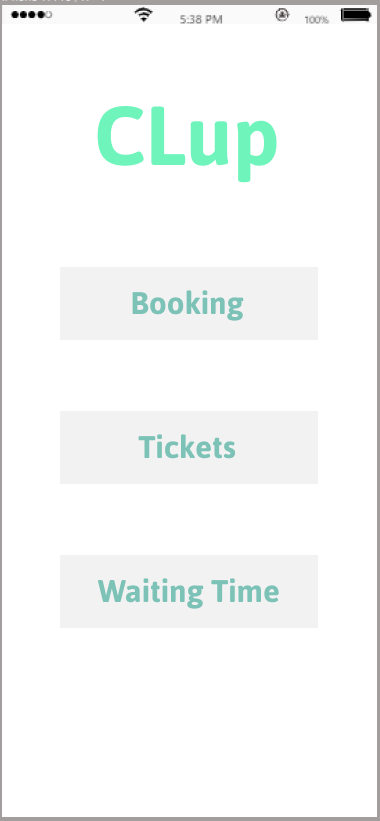
\includegraphics[scale=0.5]{UI-Home.png}
		\caption{UI-Home}
		\label{UI-Home}
	\end{minipage}%
	\begin{minipage}[t]{0.5\linewidth}
		\centering
		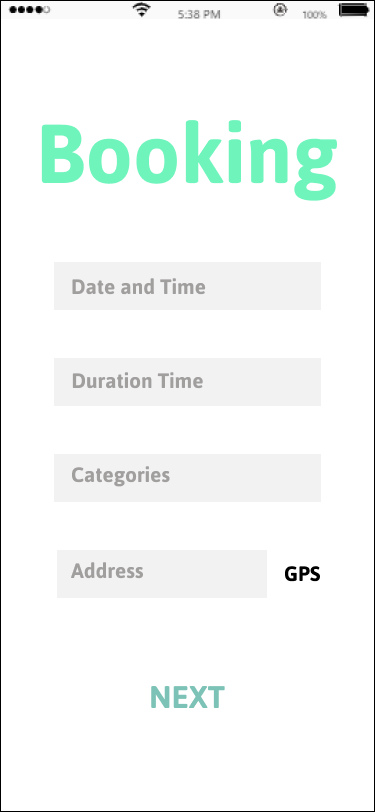
\includegraphics[scale=0.5]{UI-Booking.png}
		\caption{UI-Booking}
		\label{UI-Booking}
	\end{minipage}
\end{figure}

\begin{figure}[H] 
	\centering  
	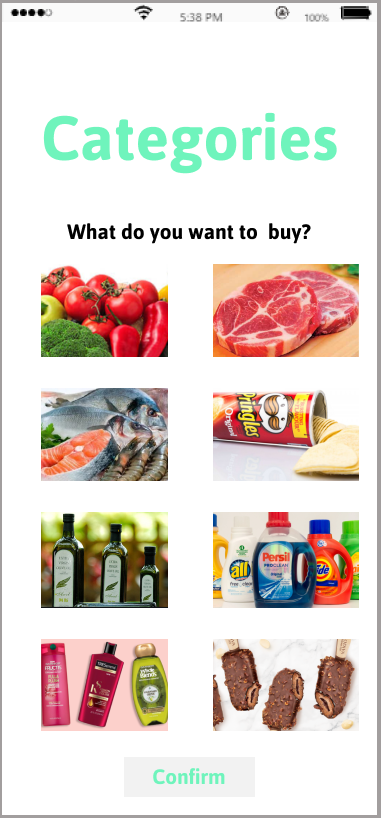
\includegraphics[scale=0.5]{UI-Category.png}
	\caption{UI-Category}
	\centering
	\label{UI-Category}
\end{figure}

\begin{figure}[H] 
	\centering  
	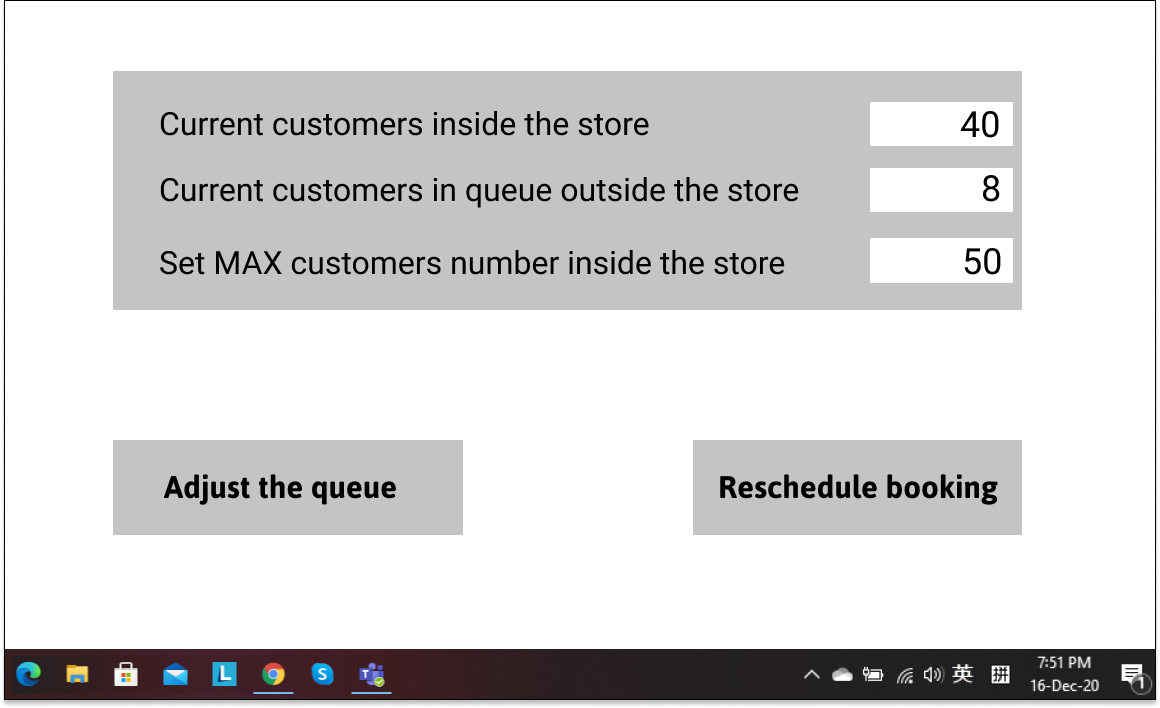
\includegraphics[scale=0.4]{UI-Dashboard.png}
	\caption{UI-Dashboard}
	\centering
	\label{UI-Dashboard}
\end{figure}


\subsection{Hardware Interfaces}
Since common users’ applications can only be accessed on mobile devices, this is the basic requirement of the user, as well as the Internet access rights to connect to the service and
a way to collect the Location data, a GPS-enabled device is required.

\subsection{Software  Interfaces}
Mobile applications require the Android operating system to run on mobile devices.
Manager dashboard requirements:
\begin{itemize}
	\item Microsoft Windows runs downloadable software
	\item Web browser to access online dashboard
\end{itemize}

\subsection{Communication Interfaces}
//TODO ZHANG


\section{Functional Requirements}
\subsection{Use Cases}

\begin{figure}
	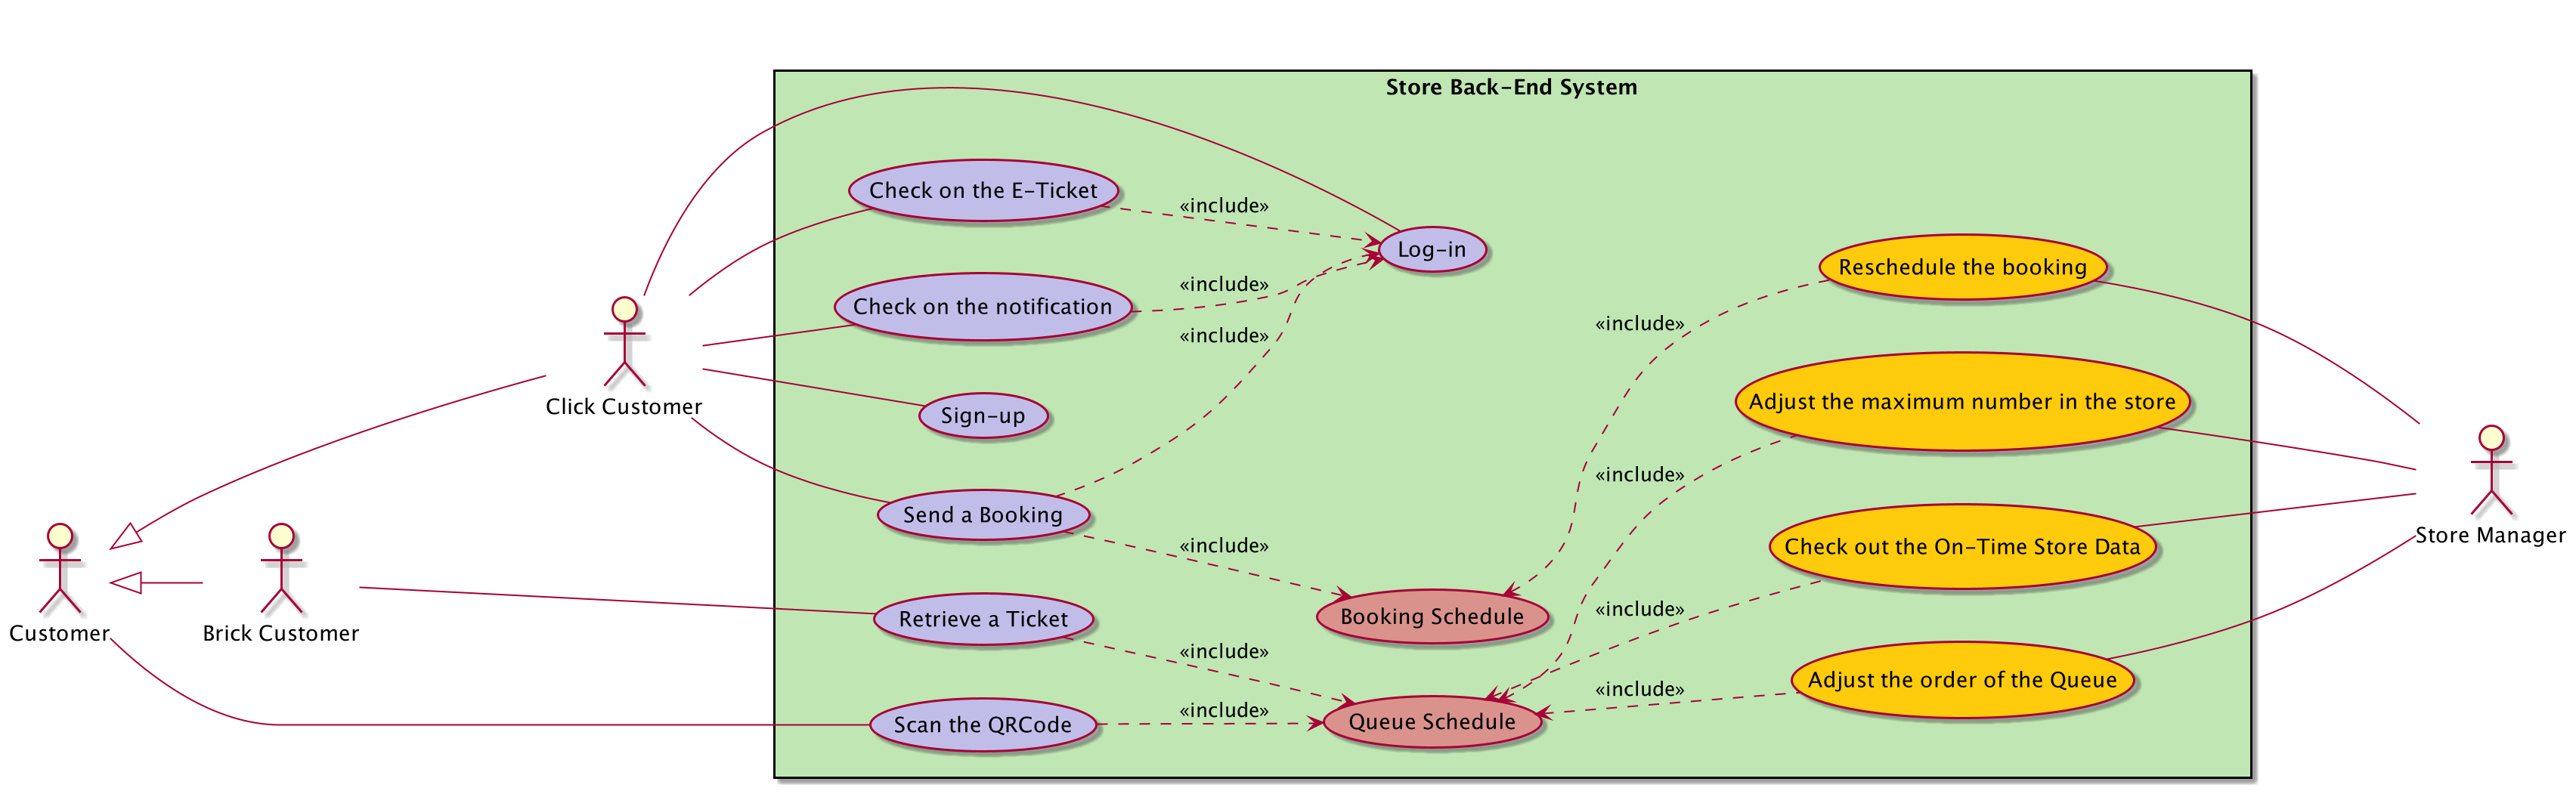
\includegraphics[angle=90,scale=0.17]{usecase_diagram.png}
	\centering
	\caption{CLup Use Case Diagram}
	\label{Use Case}
\end{figure}

\subsubsection{Click Customer’s perspective}
The following tables describe the use cases from the perspective of the  \hyperref[Definitions]{Click Customer}.
\begin{center}
	\begin{tabular}{p{0.22\textwidth}|p{0.78\textwidth}}
		\multicolumn{2}{c}{\large \textbf{Sign-up}} \\[3mm] 
		\hline \\
		Actors &  Unregistered Click Customer \\[3mm]
		Description & A new customer who wants to visit the store by booking, can register himself using the application  \\[3mm] 
		Pre-Condition & The  customer has a smart phone with Android or IOS system \\[3mm]
		Flow of events & 
		\begin{enumerate}
			\item The customer download and install the CLup application
			\item The customer open the Clup application and click the "Register" button
			\item The CLup application show a form with username, password, confirm password fields and a submit button
			\item The customer fill in the form and click the submit button
			\item The back-end system validates data and restore this data in the CRM database.
			\item The CLup application turns back automatically to the log-in page. 
		\end{enumerate}  \\[3mm]
	
		Post-Conditions & The customer now is registered in system, can do the following operations. \\[3mm]
		Exceptions & If the data inserted are not correct, the flow of events will restart from point 3.\\[3mm] 
	\end{tabular}
\end{center}

\begin{center}
	\begin{tabular}{p{0.22\textwidth}|p{0.78\textwidth}}
		\multicolumn{2}{c}{\large \textbf{Log-in}} \\[3mm] 
		\hline \\
		Actors &  Click Customer \\[3mm] 
		Description &  If the Click Customer want to do following operation, they have to log-in first  \\[3mm]  
		Pre-Condition &  The Click Customer have already registered, and input their username and password correctly \\[3mm] 
		Flow of events & 
		\begin{enumerate}
			\item The Click Customer open the CLup application.
			\item The system will show a form with username and password fields.
			\item The customer completes this form with the correct information and clicks the Log-in button.
			\item After the back-end system validated the account, the system will enter the main page automatically.
		\end{enumerate}
		\\[3mm] 
		Post-Conditions & The Click Customer is logged-in the app, and he can do the following operations.\\[3mm] 
		Exceptions & If the account info is not correct, the flow of events will restart from point 2.\\[3mm] 
	\end{tabular}
\end{center}

\begin{center}
	\begin{tabular}{p{0.22\textwidth}|p{0.78\textwidth}}
		\multicolumn{2}{c}{\large \textbf{Send a booking}} \\[3mm] 
		\hline \\
		Actors &  Click Customer \\[3mm] 
		Description &   After the Log-in, the Click Customer can use this function to book their visit.\\[3mm]  
		Pre-Condition &  Already Logged-in. \\[3mm] 
		Flow of events & 
		\begin{enumerate}
			\item The customer clicks on the book button on the main page.
			\item The system will show a form with the available visit date/time, the approximate expected duration of the visit, the categories of items they intend to buy, and the Current Place fields.
			\item The customer completes this form with the correct information. For the Current Place field, if they want, they can click on the button near the fields so that the GPS model will provide the Current Place information. 
			\item The customer clicks on the Submit button.
			\item After the back-end system validated the information, the system will store this booking on the booking schedule database. This page will show a "book successful" String and automatically go back to the main page. 
		\end{enumerate}
		\\[3mm] 
		Post-Conditions & After the booking schedule system completes the schedule, the Customer will receive the E-Ticket and the notifications. They can check on this via the following operations.\\[3mm] 
		Exceptions & If this booking is not successful, this page does not go back to the main page, the flow of events will restart from point 2.\\[3mm] 
	\end{tabular}
\end{center}

\begin{center}
	\begin{tabular}{p{0.22\textwidth}|p{0.78\textwidth}}
		\multicolumn{2}{c}{\large \textbf{Check on the E-Tickets}} \\[3mm] 
		\hline \\
		Actors &  The Click Customer \\[3mm] 
		Description &  The customer can click on the "Check on the E-Ticket" button at all times to check on their bookings. \\[3mm]  
		Pre-Condition &  They have to log-in first.\\[3mm] 
		Flow of events & 
		\begin{enumerate}
			\item The customer clicks on the "Check on the E-Ticket" button on the main page.
			\item This page shows all valid E-Ticket and the historical no valid E-ticket.
			\item The customer clicks on the E-Ticket they are interested in.
			\item The E-Ticket is in PDF format, the application will jump to the PDF reader to open it.
		\end{enumerate}
		\\[3mm] 
		Post-Conditions & After reading it, the system will still stop on the E-Ticket page.
		\\[3mm] 
		Exceptions & If they did not book any visit,  this page would show the "No booking yet" field.\\[3mm] 
	\end{tabular}
\end{center}

\begin{center}
	\begin{tabular}{p{0.22\textwidth}|p{0.78\textwidth}}
		\multicolumn{2}{c}{\large \textbf{Check on the Notifications}} \\[3mm] 
		\hline \\
		Actors &  The Click Customer \\[3mm] 
		Description &  The customer can click on the "Check on the Notification" button at all times.  \\[3mm]  
		Pre-Condition &  They have to log-in first.\\[3mm] 
		Flow of events & 
		\begin{enumerate}
			\item The customer clicks on the "Check on the Notification" button on the main page.
			\item This page shows all notifications, and the unread notifications will mark with a little red icon.
			\item The customer clicks on the notification they are interested in. If they read an unread notification, the little red icon will cancel.
		\end{enumerate}
		\\[3mm] 
		Post-Conditions & After reading it, the system will still stop on this page, and if they clicked on all unread notifications so that there is no unread notification, the "Check on the Notification" button on the main page will become the standard color.\\[3mm] 
		Exceptions & If they did have any notifications,  this page would show the "No notification yet" field.  \\[3mm] 
	\end{tabular}
\end{center}


\subsubsection{Brick Customer’s perspective}
The following table describe the use cases from the perspective of the  \hyperref[Definitions]{Brick Customer}.
\begin{center}
	\begin{tabular}{p{0.22\textwidth}|p{0.78\textwidth}}
		\multicolumn{2}{c}{\large \textbf{Retrieve a Ticket}} \\[3mm] 
		\hline \\
		Actors &  The Brick Customerw \\[3mm] 
		Description & The Brick Customer has to go to the store and retrieve the paper Ticket on the \hyperref[Definitions]{Tickets Hand-Out Machine}.   \\[3mm]  
		Pre-Condition &  The Tickets Hand-Out Machine is available.\\[3mm] 
		Flow of events & 
		\begin{enumerate}
			\item The Brick Customer goes to the store and finds the Tickets Hand-Out Machine.
			\item Click on the "Retrieve the Ticket" button on the machine.
			\item After the Back-End system schedule it in the Queue Schedule system, the machine prints the Ticket.
			\item The Brick Customer retrieves the Ticket.
		\end{enumerate}
		\\[3mm] 
		Post-Conditions & \\[3mm] 
		Exceptions & \\[3mm] 
	\end{tabular}
\end{center}


\subsubsection{Customer's perspective}
All kinds of customers have to do this operation.
\begin{center}
	\begin{tabular}{p{0.22\textwidth}|p{0.78\textwidth}}
		\multicolumn{2}{c}{\large \textbf{Scan the QRCode}} \\[3mm] 
		\hline \\
		Actors &   The Click  \& Brick Customer \\[3mm] 
		Description & All customers have to scan the QRCode when they enter and exit the store.\\[3mm]  
		Pre-Condition &  They hold the Ticket.\\[3mm] 
		Flow of events & 
		\begin{enumerate}
			\item The customer shows the QRCode in the Ticket.
			\item Scan it on the \hyperref[Definitions]{QR Code Scanned Machine} when they enter the store.
			\item Scan it on the QR Code Scanned Machine when they leave the store.
		\end{enumerate}
		\\[3mm] 
		Post-Conditions & After they scan the QR Code when they leave, the QRCode is invalid. \\[3mm] 
		Exceptions & \\[3mm] 
	\end{tabular}
\end{center}



\subsubsection{Store Manager’s perspective}
The following tables describe the use cases from the perspective of the \hyperref[Definitions]{Store Manager}.

\begin{center}
	\begin{tabular}{p{0.22\textwidth}|p{0.78\textwidth}}
		\multicolumn{2}{c}{\large \textbf{Check out the On-Time Store Data}} \\[3mm] 
		\hline \\
		Actors &   The Store Manager \\[3mm] 
		Description &  The Store Manager can view the \hyperref[Definitions]{On-Time Store Data} at any time. \\[3mm]  
		Pre-Condition & The Back-End system is working well.
		 \\[3mm] 
		Flow of events & 
		\begin{enumerate}
			\item The manager enters the manage page.
			\item The page shows all On-Time Store Data right on the main page.
		\end{enumerate}
		\\[3mm] 
		Post-Conditions & \\[3mm] 
		Exceptions & \\[3mm] 
	\end{tabular}
\end{center}



\begin{center}
	\begin{tabular}{p{0.22\textwidth}|p{0.78\textwidth}}
		\multicolumn{2}{c}{\large \textbf{Reschedule the booking}} \\[3mm] 
		\hline \\
		Actors &   The Store Manager \\[3mm] 
		Description & When the manager considers some area is too crowded, the queue is too long, or other necessary cases make them have to reschedule some customers' booking, they can do this operation. \\[3mm]  
		Pre-Condition & The Back-End system is working well, there is at least one modifiable booking.  \\[3mm] 
		Flow of events & 
		\begin{enumerate}
			\item The manager enters the manage page.
			\item Click on the "Reschedule Booking" button.
			\item The system jumps to the booking page that shows all the bookings.
			\item The system marks the modifiable booking as red color (the bookings with departure time after the current time are modifiable)
			\item The manager clicks or searches for a booking or selects some bookings.
			\item The manager modifies the modifiable booking and clicks the "Confirm" button.
			\item Wait for the Back-End system to deal with all operations and update the booking page automatically.
		\end{enumerate}
		\\[3mm] 
		Post-Conditions & The Back-End system will send the notification and update the E-Ticket for the Click Customer. \\[3mm] 
		Exceptions & If the Store Manager submits the wrong information, or this process is not successful, the flow of events will restart from point 3. \\[3mm] 
	\end{tabular}
\end{center}



\begin{center}
	\begin{tabular}{p{0.22\textwidth}|p{0.78\textwidth}}
		\multicolumn{2}{c}{\large \textbf{Adjust the order of the Queue}} \\[3mm] 
		\hline \\
		Actors & The Store Manager  \\[3mm] 
		Description & When the manager views some area is too crowded, they want customers who will visit these areas to enter the store later, or other necessary cases, they can do this operation to adjust the queue order.  \\[3mm]  
		Pre-Condition &  The Back-End system is working well, and the queue is more than two customers. \\[3mm] 
		Flow of events & 
		\begin{enumerate}
			\item The manager enters the manage page.
			\item Click on the "Adjust the queue order" button.
			\item The system jumps to the queue schedule page that shows the current queue in visualization mode.
			\item The manager clicks or searches for a kind of customer or selects some customers.
			\item The manager modifies the queue order and clicks the "Confirm" button.
			\item Wait for the Back-End system to deal with all operations and update the queue schedule page automatically.
		\end{enumerate}
		\\[3mm] 
		Post-Conditions & After this operation, the \hyperref[Definitions]{Digital Counterpart} will call the customer's queue number according to the new queue order.\\[3mm] 
		Exceptions & If the Store Manager submits the wrong information, or this process is not successful, the flow of events will restart from point 3.
		\\[3mm] 
	\end{tabular}
\end{center}


\begin{center}
	\begin{tabular}{p{0.22\textwidth}|p{0.78\textwidth}}
		\multicolumn{2}{c}{\large \textbf{Adjust the maximum number in the store}} \\[3mm] 
		\hline \\
		Actors & The Store Manager  \\[3mm] 
		Description & When the manager considers there are too many/few people in the store, they can do this operation to regulate the influx of people in the building.
		\\[3mm]  
		Pre-Condition & The Back-End system is working well. \\[3mm] 
		Flow of events & 
		\begin{enumerate}
			\item The manager enters the manage page.
			\item Just modify the maximum number in the store value on the main page.
		\end{enumerate}
		\\[3mm] 
		Post-Conditions & If the current number is more than the maximum, the Digital Counterpart will stop to call the next customer until the current number few than the maximum. Instead, when the current number is fewer than the maximum, the Digital Counterpart will call fastly, until they are equal.
		\\[3mm] 
		Exceptions & If the Store Manager submits the wrong information, or this process is not successful, the maximum value will just come back to the previous value. \\[3mm] 
	\end{tabular}
\end{center}

\subsubsection{Sequence Diagram}
We have integrated the sequence diagrams from the perspective of the customer and store manager, respectively.

From the customer's perspective Fig.\ref{Sequence Diagram Customer}, two kinds of customers are independent and do not interfere. The queue schedule function calls the queue number via the Digital Counterpart, and the customer has to view or listen well their queue number. When their number is called, they scan their QRCode.

From the manager's perspective Fig.\ref{Sequence Diagram Manager}, their four operations are independent and do not interfere with each other.


\begin{figure}
	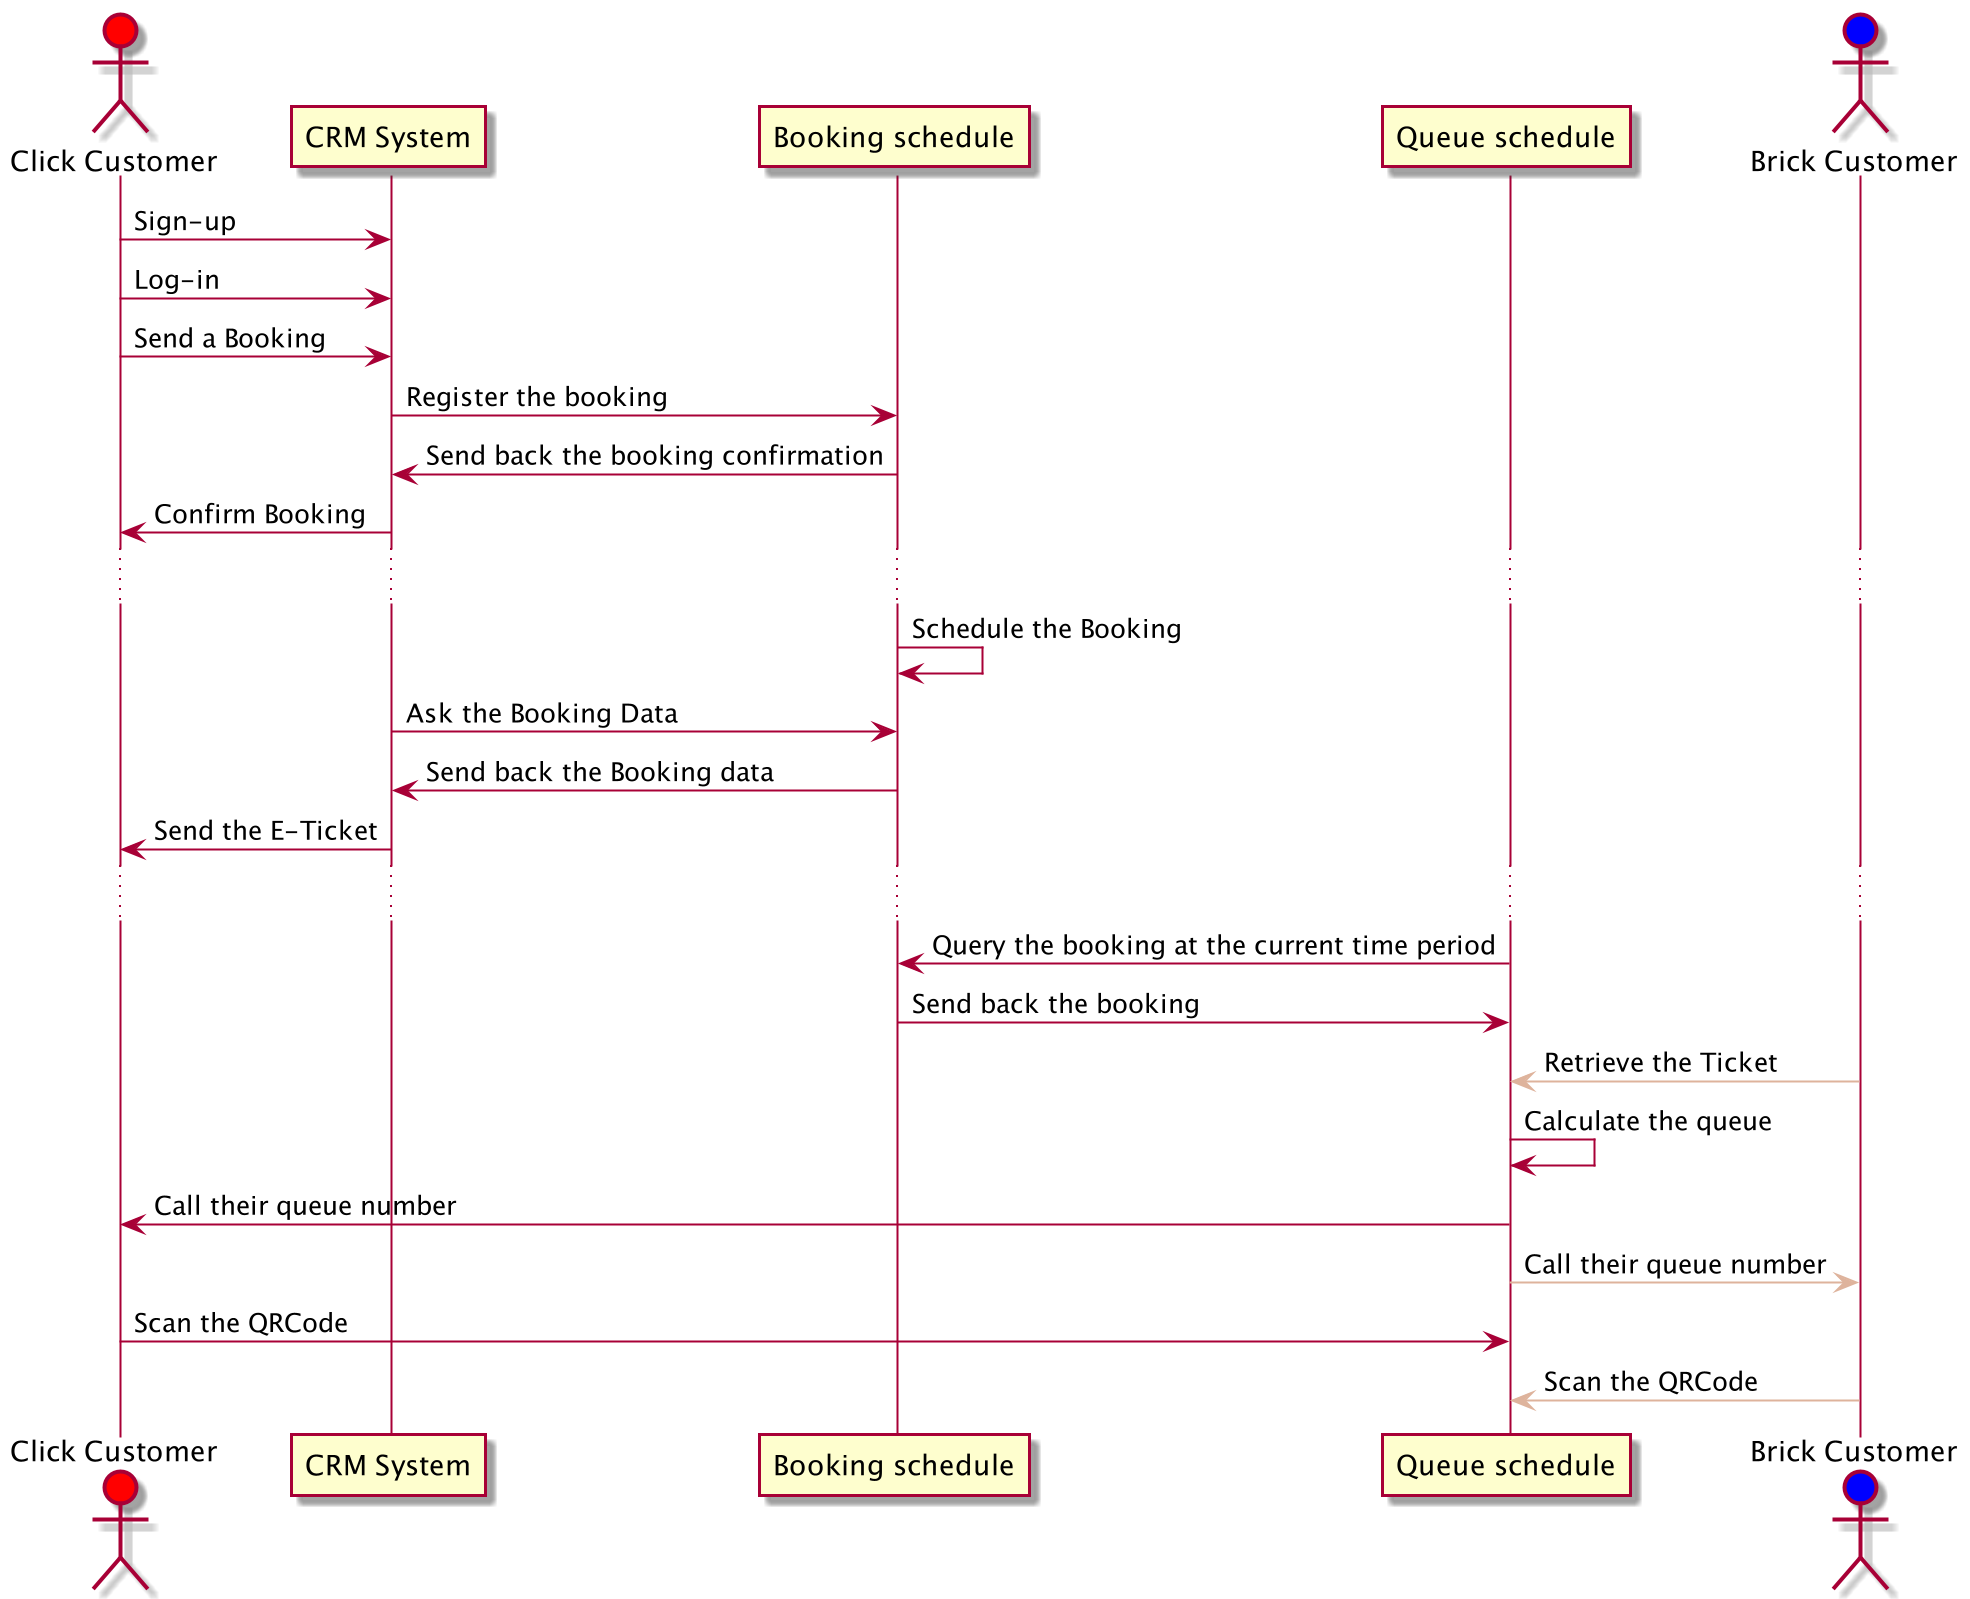
\includegraphics[scale=0.22]{sequence_diagram_customer.png}
	\centering
	\caption{Customers' Sequence Diagram}
	\label{Sequence Diagram Customer}
\end{figure}

\begin{figure}
	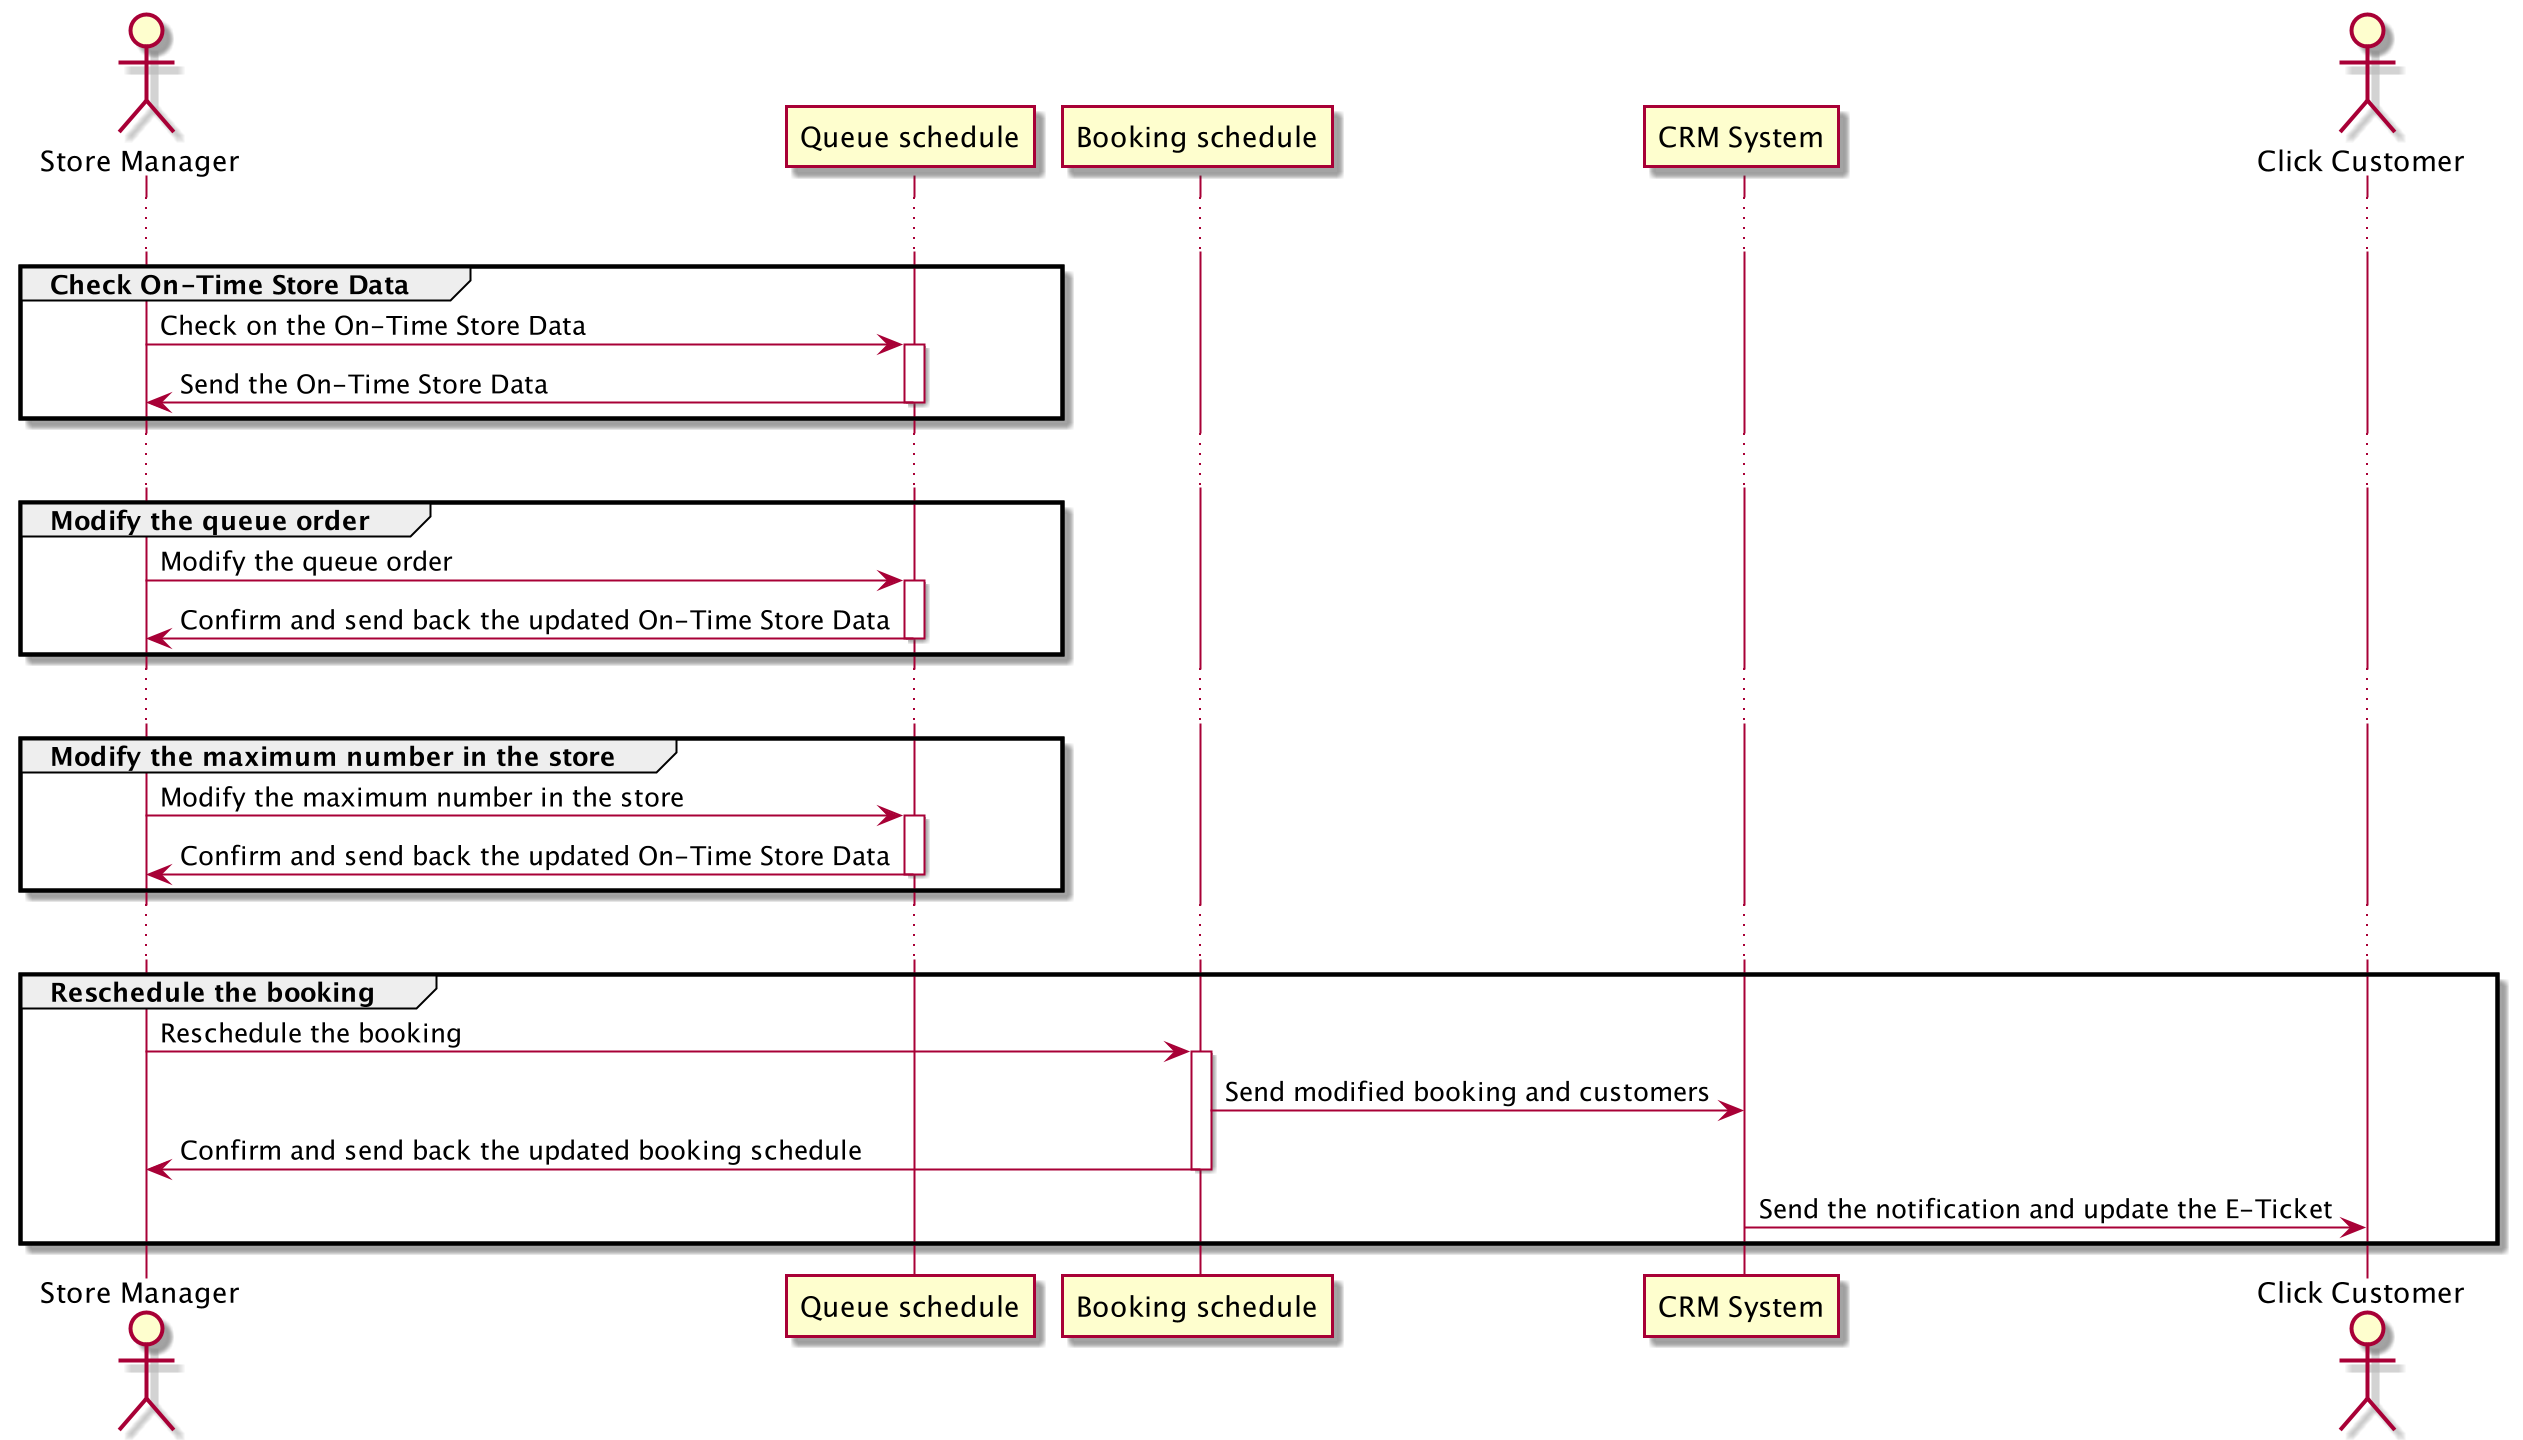
\includegraphics[scale=0.18]{sequence_diagram_manager.png}
	\centering
	\caption{Manager's Sequence Diagram}
	\label{Sequence Diagram Manager}
\end{figure}


\subsubsection{Scenarios}

In order to describe these processes more vividly, we give three scenarios from three perspectives. 

\textbf{Scenario 1 - Leonardo lives in a small town with a severe epidemic}: Leonardo, an excellent researcher, loves science, and he studies hard every day. His life is peaceful and happy in that small town. On a cold rainy day, a horrifying thing happened, his town found the COVID-19 cases! All people are terrified, and the mayor urges everyone not to go out. At this time, Leonardo cannot go to his university. Even he hardly goes out except going to the supermarket to buy food. In this challenging time, he discovered that the local supermarket "EsseCorta" was as crowded as usual, and there were also many people gathering. Even because other stores closed, the supermarket was even more crowded. To resolve this problem, Leonardo called on Essecorta to let everyone use CLup to reasonably organize shopping orders. The Essecorta owner was pleased, so within a few days, the system was deployed well.
Now Leonardo does not have to take the risk any more in Essecorta. Every weekend, he books a visit on Monday morning at 9:30. Cause lives near it, so from the E-Ticket, Leonardo has to depart from 9:10. When he arrives, he found he even does not have to wait. The Digital Counterpart calls his queue number immediately. He takes out the E-Ticket, scans his QRCode, enters the supermarket, and following the Planned Roadmap on the E-Ticket. How to say? Such convenience! When he bought all items he wants, he rescans the QRCode at the exit and goes back home happy.


\textbf{Scenario 2 - A lovely Nonna in the same town}: Nonna Angola live in this town much year. Facing this epidemic, she was very calm. She believes that this country has experienced many incidents, and people can handle the epidemic. Her life is simple, a coffee in the Morning, a Tea in the evening, that is all. She loves her simple life, and she does not want to change anything. A day, she goes to the supermarket like usual day, the store manager tells her to take a Ticket from a machine, this machine has only a simple button like this lovely Nonna's life, this button is huge, almost occupied all space of the screen, to Nonna, it is not very difficult to use. After getting her Ticket, Nonna waits for the Digital Counterpart to call her number. A few seconds later, Nonna enters the market. The store manager helps her scan the QRCode when she enters and leaves the market.


\textbf{Scenario 3 - The manager who want everyone safe}: Luca is a store manager. He was a bus driver before, but the cause of this unfortunate time, his bus was stopped, he had to find another job. The Essecorto owner found him because the driver has to keep every passager safe, so this job too! He has to look at the market at all times. One day, he finds that there are many people in the Gelato area. He realizes that it is not a good thing, so he reduces the store's maximum number. After a few minutes,  he finds that is not working, other areas have a few people, but the Gelato area still crowed. Why? Maybe this day has many children like Gelato, and these children did not book this visit. Instead, they all piked the Tiket on the Machine, so the system did not monitor all this. Then Luca decided to adopt plan B. He checks the queue schedule and puts the customers who are also visiting the Gelato area later. Five minutes later, other managers tell him the adjustment is not enough, so Luca decided to take the last resort - reschedule the Gelato's customers' booking! He opens the booking schedule page and searches the keyword "Gelato" and modifies all valid results' customers' booking and postpones this for about 1 hour. Finally, ten minutes later, this area was clean. He did an excellent job!


\subsection{Mapping on requirements}
\subsubsection{$G_1$ : Allows store managers to regulate the influx of people in the building}


\textbf{- Requirements:}
\begin{itemize}
	
	\item $R_7$: The Store Manager shall be able to Check out the On-Time Store Data.
	\item $R_8$: The Store Manager shall be able to Adjust the maximum number of people in the store. 
	\item $R_9$: The Store Manager shall be able to Adjust the order of the queue.
	\item $R_{10}$: The Store Manager shall be able to Check and reschedule the booking. 
	\item $R_{12}$: The Store Back-End System shall be able to received and schedule the click customers’ book. The scheduling must refer to the duration time of each Customer and the categories of items that the Customer intends to buy.
	\item $R_{15}$: The Store Back-End System shall send a notification and update the E-Ticket to the Customer when their book is rescheduled. 
	\item $R_{17}$: The Store Back-End System shall analyze the history visit data and mark the Long-Term Customers. 
	\item $R_{18}$: The Store Back-End System shall be able to Calculate and store the On-Time Store Data.
	\item $R_{19}$: The Store Back-End System shall schedule or reschedule the queue order from click customer’s book and the brick customer's retrieved ticket.
	\item $R_{20}$: The Store Back-End System shall be able to Control the Digital Counterpart and display the queue number. 
	\item $R_{21}$: The Store Back-End System shall be able to receive the information from the QR Code Scanned Machine. Receive the information from the Tickets Hand-Out Machine. 
\end{itemize}


\textbf{- Domain Assumptions:}
\begin{itemize}
	\item $D_4$ : If something unexpected happens, the store manager can reasonably adjust the maximum number of people in the store or reschedule the queue \& Customer's book.
	\item $D_5$ : If someone’s booking is rescheduled, he can find the notification in time and set off according to the updated E-Ticket.
\end{itemize}


\subsubsection{$G_2$ : Saves people from having to line up and stand outside of stores for hours on end}

\textbf{- Requirements:}
\begin{itemize}
	\item $R_1$: Each Click Customer shall be able to sign-up and Log-in.
	\item $R_2$: Each Click Customer shall be able to book a visit.
	\item $R_3$: Each Click Customer shall be able to check on the E-Ticket.
	\item $R_4$: Each Click Customer shall check on the store manager's notification when their book is rescheduled.
	\item $R_5$: Each Brick Customer shall be able to retrieve the Ticket from the Tickets Hand-Out Machine and wait for the Digital Counterpart to call them.
	\item $R_6$: Each Customer shall scan the QR Code at QR Code scanned machine when they enter and leave the store.
	\item $R_{11}$: The Store Back-End System shall send the available time/date to the click customers. 
	\item $R_{12}$: The Store Back-End System shall be able to received and schedule the click customers’ book. The scheduling must refer to the duration time of each Customer and the categories of items that the Customer intends to buy.
	\item $R_{13}$: The Store Back-End System shall calculate the time from the click customer’s departure place to the store and put the estimated departure time on the E-Ticket. 
	\item $R_{15}$: The Store Back-End System shall send a notification and update the E-Ticket to the Customer when their book is rescheduled. 
	\item $R_{16}$: The Store Back-End System shall be able to store the Customer’s data.
	\item $R_{17}$: The Store Back-End System shall analyze the history visit data and mark the Long-Term Customers. 
	\item $NR_1$:The time from the click customer's departure place to the store that calculates from the Store Back-End System must be precise enough to avoid the Customer arriving at the store too early/late.
	\item $NR_2$:The Store Back-End System must schedule the queue reasonably to minimize the wait time.
	\item $NR_3$:The Store Back-End System must mix the book and brick customer's retrieved ticket reasonably to allow the click customers to enter the store near the book time by avoiding making the brick customers wait too long.
	\item $NR_4$:Cause everyone needs to do grocery shopping, the software for the click customer should be simple enough to use.
\end{itemize}

\textbf{- Domain Assumptions:}
\begin{itemize}
	\item $D_1$ : Everyone will leave the departure place at the departure time indicated by the system.
	\item $D_2$ : Everyone who leaves on time can arrive at the store on time.
	\item $D_3$ : After shopping, everyone can leave the store in time according to their estimated time.
	\item $D_5$ : If someone’s booking is rescheduled, he can find the notification in time and set off according to the updated E-Ticket.
	\item $D_6$ : Everyone can consciously scan the QR code at the entrance and exit.
	\item $D_8$ : If possible, everyone tries to book the visit via the application(be a \hyperref[Definitions]{Click Customer}) instead of picking up tickets on the spot(not be a \hyperref[Definitions]{Brick Customer}).
\end{itemize}


\subsubsection{$G_3$ : The application plan visits in a finer way to allow more people in the store, at the same time, let the customer occupy different spaces in the store to keep enough distance between them}

\textbf{- Requirements:}
\begin{itemize}
	\item $R_{12}$: The Store Back-End System shall be able to received and schedule the click customers’ book. The scheduling must refer to the duration time of each Customer and the categories of items that the Customer intends to buy.
	\item $R_{14}$: The Store Back-End System shall Plan and put the Store Planned Roadmap on the E-Ticket Send the E-Ticket to the click customers. 	
	\item $R_{17}$: The Store Back-End System shall analyze the history visit data and mark the Long-Term Customers. 
\end{itemize}


\textbf{- Domain Assumptions:}
\begin{itemize}
	\item $D_3$ : After shopping, everyone can leave the store in time according to their estimated time.
	\item $D_7$ : Everyone can follow the \hyperref[Definitions]{Planned Roadmap} in the store.
\end{itemize}


\subsubsection{Traceability Matrix   }


\begin{center}
	\setlength{\tabcolsep}{10pt} 
	\renewcommand{\arraystretch}{1.5}
	\begin{tabular}{ |c|c|c| } 
		\hline
		\textbf{Goals} & \textbf{Requirements} & \textbf{Domain Assumptions} \\
		\hline
		\hline
		$G_1$ & \makecell{$R_7$, $R_8$, $R_9$, $R_{10}$, $R_{12}$, $R_{15}$, \\ $R_{17}$, $R_{18}$, $R_{19}$,  $R_{20}$, $R_{21}$} & $D_4$, $D_5$ \\
		\hline
		$G_2$ &  \makecell{$R_1$, $R_2$, $R_3$, $R_4$, $R_5$, $R_6$, \\ $R_{11}$, $R_{12}$, $R_{13}$, $R_{15}$,  $R_{16}$, $R_{17}$, \\  $NR_1$, $NR_2$, $NR_3$, $NR_4$}  &  $D_1$, $D_2$, $D_3$, $D_5$, $D_6$, $D_8$\\
		\hline
		$G_3$ & $R_{12}$, $R_{14}$, $R_{17}$ & $D_3$, $D_7$ \\
		\hline
	\end{tabular}
\end{center}

In summary, we proved the \textbf{Requirements Completeness} of our system, so that \textbf{R and D   $\models$   G}.




\section{Performance Requirements}

The Click Customer must have a smartphone with the Android or IOS operation system. When they open the book a visit page, the Back-End system has to send them the available data/time within 1 second. After they send the form, the Back-End system has to confirm it within 5 seconds. And then, the Back-End system has to schedule this booking, generate QRCode, Queue Number, Estimated departure time, and Planned Roadmap, integrate them to the E-Ticket, and send back the E-Ticket so soon as possible. Cause calculate the Planned Roadmap Operation has to wait for the other Customer's data, so this operation can not complete quickly. However, //TODO
it must send the E-Ticket to the Customer 24 hours before departure. 

For the Brick Customer, no need for them to hold any personal drives. They have to learn how to use the Ticket Hand-Out Machine. As the range of users includes all demographics, this machine has to be easy enough to use. When the Brick Customer retrieves the Ticket, the paper Ticket has to print in 1 second.

For the Store Manager, their management system will implement in a PC with a stable network connection. When they do any operation, this system has to react in 5 seconds.

For the Back-End system, we will buy an Amazon EC2 IaaS to implement it. This system will communicate with all other ends, so we have to keep this system always working well, cause it is Iaas, we still have to keep our software function, the KPI is every month the unavailable service time does not exceed 1 hour.


\section{Design Constraints}
\subsection{Standards compliance}

Our system complies with the following standards
\begin{itemize}
	\item 
\end{itemize}


\subsection{Hardware limitations}

For our Click Customer application to run well on smartphones, we must follow the following hardware limitations:
\begin{itemize}
	\item 
\end{itemize}

For our Management System run on the PC, the hardware limitations are:
\begin{itemize}
	\item 
\end{itemize}

Furthermore, the hardware limitation of the Back-End System are:
\begin{itemize}
	\item 
\end{itemize}


//TODO KONG
section{Software System Attributes}
\subsection{Reliability} 

\subsection{Availability}

\subsection{Security} 
Since the collected user data is very sensitive, the user’s privacy must be considered during the entire data exchange process between the user and the system, and also between the system and the third party. The data stored in the system must be encrypted, and the municipality’s password must also be hashed before storing in Database.\\

\subsection{Maintainability} The code must be written by Java, in order to let other developers easily understand and edit it. It also need to be well commented corresponding to the code in case of future issues.\\

\subsection{Portability} The mobile application must be supported by Android and iOS operating systems. The web application must run in various operating systems: Windows, Linux, Mac.\\




//TODO ZHANG
\chapter{Formal Analysis Using Alloy}
Each user is uniquely identified by a username
The On-Time number of peoble is euqal or min than max number



\chapter{Effort Spent}

\begin{itemize}
	\item \textbf{Kong Xiangyi}
	\begin{center}
		\begin{tabular}{ |c|c|c| } 
			\hline
			Date & Task & Hours \\
			\hline
			\hline
			2020/10/10 & Group discussion project plan & 4h \\ 
			\hline
			2020/10/31 & Modified the purpose and scope of the RASD & 2h \\ 
			\hline
			2020/11/14 & Drawn the state diagram in the Section 2.1.1 & 2h \\ 
			\hline
			2020/11/26 & Design and drawn the UI in section 3.1.1 & 2h \\
			\hline
			2020/12/5 & Completed the User Interface requirement & 3h \\
			\hline
			2020/12/6 & Inspected the section 2 & 1h \\
			\hline
			2020/12/10 & Wrote the overview & 1h \\
			\hline
			2020/12/18 & Completed the section 3.4 and fixed the problem in chapter 3 & 2h \\
			\hline
			//TODO KONG
		\end{tabular}
	\end{center}


	\item \textbf{Zhang Yuedong}
	\begin{center}
		\scalebox{0.9}{
		\begin{tabular}{ |c|c|c| } 
			\hline
			Date & Task & Hours \\
			\hline
			\hline
			2020/10/10 & Group discussion project plan & 4h \\ 
			\hline
			2020/10/19 & Added the project's architecture & 1h \\ 
			\hline
			2020/10/30 & Added the purpose and scope of the RASD & 2h \\ 
			\hline
			2020/11/16 & Wrote the product functions part & 4h \\ 
			\hline
			2020/11/17 & Drawn the class diagram in the Section 2.1.1  & 2h \\ 
			\hline
			2020/11/27 & Fixed the problem of the second chapter & 1h \\
			\hline
			2020/12/04 & Completed the use case, sequence, and the scenario in the Section 3.2 & 4h \\
			\hline
			2020/12/05 & Completed the Mapping on requirements in the section 3.2 & 2h \\
			\hline
			2020/12/06 & Completed the Performance Requirements & 1h \\
			\hline
		\end{tabular}}
	\end{center}
\end{itemize}



\end{document}
